% Created 2025-06-19 Thu 03:58
% Intended LaTeX compiler: pdflatex
\documentclass[12pt,xcolor=dvipsnames,presentation,aspectratio=169]{beamer}
\usepackage[utf8x]{inputenc}
\usepackage[T1]{fontenc}
\usepackage{graphicx}
\usepackage{longtable}
\usepackage{wrapfig}
\usepackage{rotating}
\usepackage[normalem]{ulem}
\usepackage{amsmath}
\usepackage{amssymb}
\usepackage{capt-of}
\usepackage{hyperref}
\usedescriptionitemofwidthas{bl}
\usepackage{ifthen,figlatex,amsmath,amstext,xspace}
\usepackage{boxedminipage,xspace,multicol}
\usepackage{subfigure}
\usepackage{fancyvrb}
\usetheme{Madrid}
\usecolortheme[named=BrickRed]{structure}
%\usepackage[colorlinks=true,citecolor=pdfcitecolor,urlcolor=pdfurlcolor,linkcolor=pdflinkcolor,pdfborder={0 0 0}]{hyperref}
\usepackage[round-precision=3,round-mode=figures,scientific-notation=true]{siunitx}
\setbeamertemplate{footline}[frame number]
\setbeamertemplate{navigation symbols}{}
\usepackage{DejaVuSansMono}
%\AtBeginDocument{
%  \definecolor{pdfurlcolor}{rgb}{0,0,0.6}
%  \definecolor{pdfcitecolor}{rgb}{0,0.6,0}
%  \definecolor{pdflinkcolor}{rgb}{0.6,0,0}
%  \definecolor{light}{gray}{.85}
%  \definecolor{vlight}{gray}{.95}
%}
\usepackage{appendixnumberbeamer}
\usepackage{relsize}
\usepackage{color,colortbl}
\definecolor{gray98}{rgb}{0.98,0.98,0.98}
\definecolor{gray20}{rgb}{0.20,0.20,0.20}
\definecolor{gray25}{rgb}{0.25,0.25,0.25}
\definecolor{gray16}{rgb}{0.161,0.161,0.161}
\definecolor{gray60}{rgb}{0.6,0.6,0.6}
\definecolor{gray30}{rgb}{0.3,0.3,0.3}
\definecolor{bgray}{RGB}{248, 248, 248}
\definecolor{amgreen}{RGB}{77, 175, 74}
\definecolor{amblu}{RGB}{55, 126, 184}
\definecolor{amred}{RGB}{228,26,28}
\usepackage[procnames]{listings}
\lstset{ %
backgroundcolor=\color{gray98},    % choose the background color; you must add \usepackage{color} or \usepackage{xcolor}
basicstyle=\tt\prettysmall,      % the size of the fonts that are used for the code
breakatwhitespace=false,          % sets if automatic breaks should only happen at whitespace
breaklines=true,                  % sets automatic line breaking
showlines=true,                  % sets automatic line breaking
captionpos=b,                     % sets the caption-position to bottom
commentstyle=\color{gray30},      % comment style
extendedchars=true,               % lets you use non-ASCII characters; for 8-bits encodings only, does not work with UTF-8
frame=single,                     % adds a frame around the code
keepspaces=true,                  % keeps spaces in text, useful for keeping indentation of code (possibly needs columns=flexible)
keywordstyle=\color{amblu},       % keyword style
procnamestyle=\color{amred},       % procedures style
language=C,             % the language of the code
numbers=none,                     % where to put the line-numbers; possible values are (none, left, right)
numbersep=5pt,                    % how far the line-numbers are from the code
numberstyle=\tiny\color{gray20}, % the style that is used for the line-numbers
rulecolor=\color{gray20},          % if not set, the frame-color may be changed on line-breaks within not-black text (e.g. comments (green here))
showspaces=false,                 % show spaces everywhere adding particular underscores; it overrides 'showstringspaces'
showstringspaces=false,           % underline spaces within strings only
showtabs=false,                   % show tabs within strings adding particular underscores
stepnumber=2,                     % the step between two line-numbers. If it's 1, each line will be numbered
stringstyle=\color{amdove},       % string literal style
tabsize=2,                        % sets default tabsize to 2 spaces
% title=\lstname,                    % show the filename of files included with \lstinputlisting; also try caption instead of title
procnamekeys={call}
}
\newcommand{\prettysmall}{\fontsize{6}{8}\selectfont}
\newcommand{\quitesmall}{\fontsize{8}{10}\selectfont}
\usepackage{tikzsymbols}
\def\smiley{\Smiley[1][green!80!white]}
\def\frowny{\Sadey[1][red!80!white]}
\def\winkey{\Winkey[1][yellow]}
\def\smileyitem{\setbeamertemplate{itemize item}{\scriptsize\raise1.25pt\hbox{\donotcoloroutermaths\color{black}$\smiley$}}}
\def\frownyitem{\setbeamertemplate{itemize item}{\scriptsize\raise1.25pt\hbox{\donotcoloroutermaths\color{black}$\frowny$}}}
\def\restoreitem{\setbeamertemplate{itemize item}[ball]}
\def\smileysubitem{\setbeamertemplate{itemize subitem}{\scriptsize\raise1.25pt\hbox{\donotcoloroutermaths\color{black}$\smiley$}}}
\def\frownysubitem{\setbeamertemplate{itemize subitem}{\scriptsize\raise1.25pt\hbox{\donotcoloroutermaths\color{black}$\frowny$}}}
\def\restoresubitem{\setbeamertemplate{itemize subitem}[ball]}
\usetheme{default}
\author{schnorr}
\date{\today}
\title{Spatio-Temporal Aggregation of StarPU multi-node traces}
\begin{document}

\urlstyle{sf}
\let\alert=\structure
\let\epsilon=\varepsilon
\let\leq=\leqslant
\let\geq=\geqslant

{%\setbeamertemplate{footline}{} 

\author{Lucas Mello Schnorr, Lucas Assis \newline Instituto de Informática, UFRGS}

\date{-- NumPex / ExaSoft / WP5 -- \newline (chez Datamove)  \newline June 19th, 2025 \\\smallskip}

\titlegraphic{\vspace{-.5cm
    
\includegraphics[scale=0.12]{./logo/ppgc.png}\hspace{2cm}
    
\includegraphics[scale=1.6]{./logo/ufrgs2.png}}}

\maketitle
\begin{frame}[label={sec:org806b622}]{Introduction \& Motivation}
\uline{StarPU-MPI}: Task Programming over Clusters of Machines Enhanced with Accelerators:
\url{https://inria.hal.science/hal-00725477}
\begin{itemize}
\item Each node generates a FXT file with timestamped events
\item Voluminous traces with all application tasks (and many other data)
\begin{itemize}
\item Start/End of states, performance metrics
\end{itemize}
\end{itemize}

\vfill\pause

Assumptions
\begin{enumerate}
\item Provide an exploratory analysis of the application/runtime behavior
\begin{itemize}
\item We don't know possible performance issues \(\to\) minimal filtering
during tracing
\item Justify performance problems with contextual information from traces
\end{itemize}
\item Trace visualization overwhelmed by the amount of data (temporal/spatial)
\begin{itemize}
\item Necessity of a visualization \(\to\) Visualizing More Performance Data
Than What Fits on Your Screen: \url{https://inria.hal.science/hal-00737651}
\end{itemize}
\end{enumerate}

\vfill\pause
\begin{block}{Problems}
(1) Too much but necessary traces; (2) Visualization scalability of space/time views
\end{block}
\end{frame}
\begin{frame}[label={sec:org13ef2c3},fragile]{Objetive \& Approach}
 \begin{enumerate}
\item Do trace aggregation before the trace visualization
\item Investigate specifically the spatial/temporal aggregation together
\item Provide a traditional space/time view
\end{enumerate}

\pause\vfill

Existing efforts within StarVZ (\url{https://cran.r-project.org/web/packages/starvz/})
\begin{center}
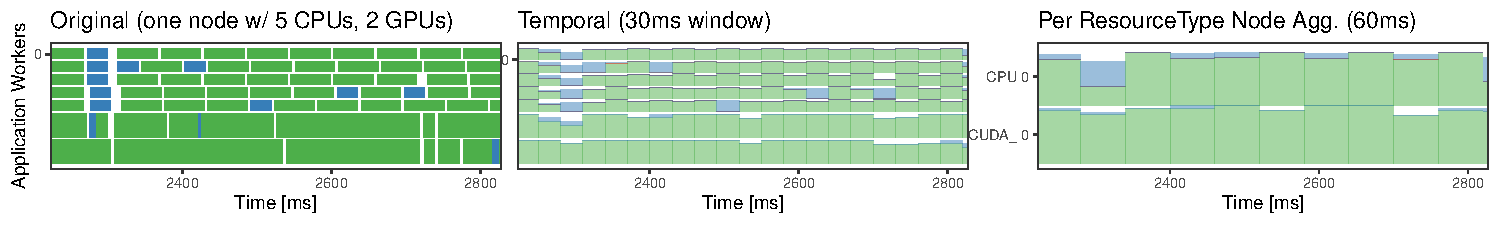
\includegraphics[width=.9\linewidth]{./agg_starvz.pdf}
\end{center}
\(\to\) It lacks spatial aggregation (i. e. aggregate nodes with similar behavior)

\pause\vfill
\begin{block}{Goal}
Explore \texttt{lpaggreg} within the context of StarVZ for StarPU traces |
Dosimont et. al. "A spatiotemporal data aggregation technique for
performance analysis of large-scale execution traces". CLUSTER 2014
\(\to\) \url{https://github.com/dosimont/lpaggreg}
\end{block}
\end{frame}
\begin{frame}[label={sec:orge965911},fragile]{Methodology \& Workflow}
 (A) In the cluster
\begin{enumerate}
\item Run the experiment in the cluster
\item Collect FXT traces
\item Run StarVZ Phase 1 script \(\to\) PARQUET (Columnar-based files)
\end{enumerate}

(B) In the laptop
\begin{enumerate}
\item Employ StarVZ R Package
\item Integrate \uline{lpaggreg} (this work)
\begin{itemize}
\item \texttt{read\_starvz}, export pjdump, micro, aggregation, viz
\end{itemize}
\end{enumerate}

\vfill\pause

(C) Evaluation
\begin{itemize}
\item Use previous StarPU traces obtained with (A)
\begin{itemize}
\item Nesi et. al. "Summarizing task-based applications behavior over
many nodes through progression clustering". PDP 2023. |
Chameleon + ExaGeoStat
\end{itemize}
\item Stress the usage of lpaggreg features (Information Loss, Complexity Reduction)
\end{itemize}
\end{frame}
\begin{frame}[label={sec:org5e20003},fragile]{Lpaggreg features (Information Loss, Complexity Reduction)}
 Integrate \uline{lpaggreg} (this work)
\begin{itemize}
\item \texttt{read\_starvz}, export pjdump, micro, aggregation, viz
\end{itemize}

%\vspace{0.2cm}
\begin{columns}
\begin{column}{0.5\columnwidth}
\scalebox{0.5}{\parbox{\linewidth}{%
\begin{center}
\begin{tabular}{rrrl}
Parameter & Gain & Loss & POpt\\
\hline
0 & 0.0411956541727119 & -1.02641907782919e-16 & FALSE\\
0.0625 & 0.173655727924065 & 0.00157655769097006 & FALSE\\
0.125 & 0.382826967688981 & 0.0249004552694742 & FALSE\\
0.1875 & 0.603343589271184 & 0.0644300849930824 & FALSE\\
0.25 & 0.615363211728487 & 0.0677042920117212 & FALSE\\
0.3125 & 0.627709273385034 & 0.0724654636070262 & FALSE\\
0.375 & 0.648086722611672 & 0.0828704306131623 & FALSE\\
0.4375 & 0.686311544823401 & 0.108093646729556 & FALSE\\
0.5 & 0.927290907242805 & 0.305838193382574 & TRUE\\
0.5625 & 0.929053986692192 & 0.307990944412131 & FALSE\\
0.625 & 0.93092906631553 & 0.311047076192813 & FALSE\\
0.6875 & 0.948104037152438 & 0.342731084421385 & FALSE\\
0.8125 & 0.949305929084811 & 0.34671405810594 & FALSE\\
0.875 & 0.953750338312438 & 0.374181737848363 & FALSE\\
0.9375 & 0.99223795542665 & 0.859582936312456 & FALSE\\
1 & 1 & 1 & FALSE\\
\end{tabular}
\end{center}
}}
\end{column}
\begin{column}{0.5\columnwidth}
\begin{center}
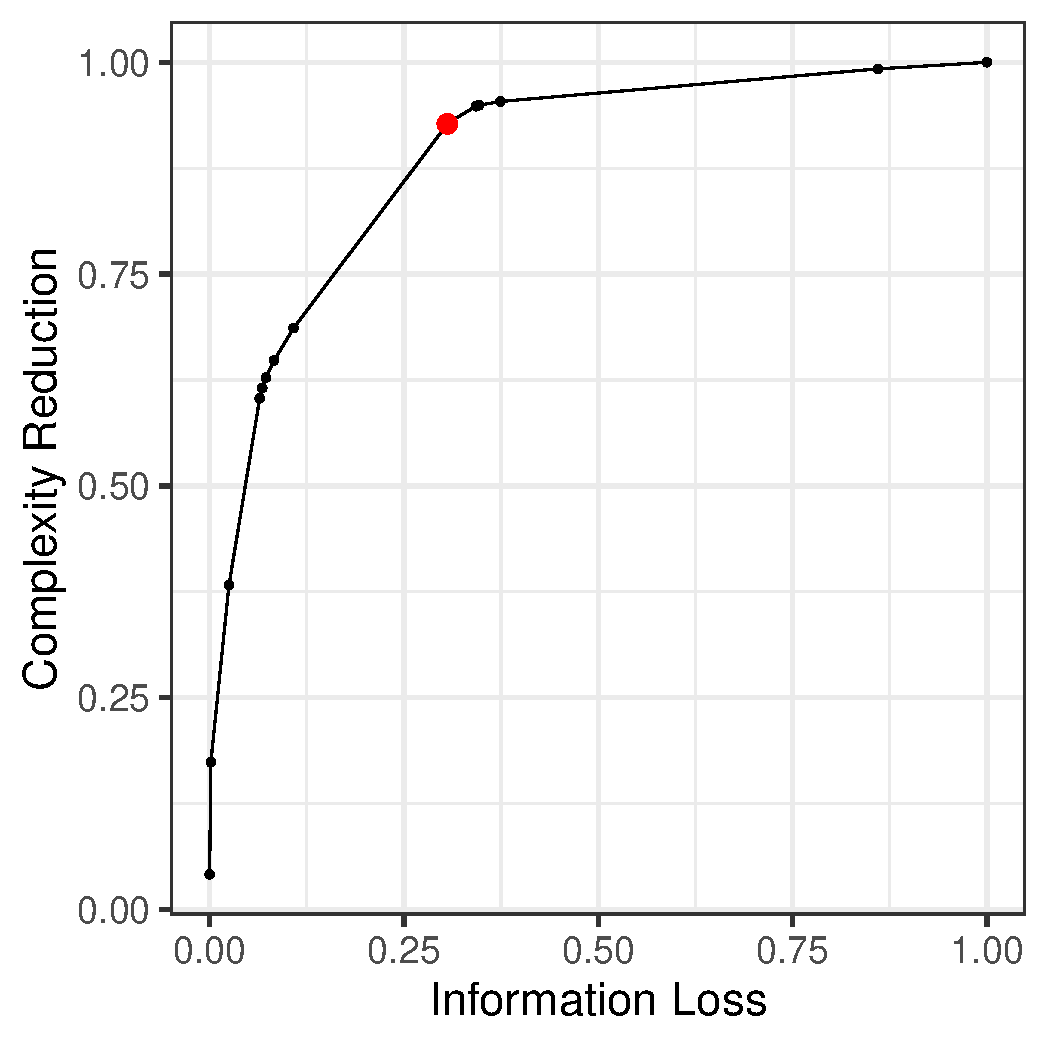
\includegraphics[width=.6\linewidth]{./p_example.pdf}
\end{center}
\end{column}
\end{columns}
Each spatio/temporal aggregation provides several views
\begin{itemize}
\item One for each \alert{Parameter}: 0 means minimal aggregation; 1 means full aggregation
\item Each parameter represent a tradeoff (with an ``ideal tradeoff'', see \alert{POpt})
\end{itemize}
\end{frame}
\begin{frame}[label={sec:org13d4819},fragile]{Case studies (Chameleon Dense LU Facto. and ExaGeoStat)}
 \texttt{2W+DIF}: 30 nodes, 2 GPUs each, two faulty nodes with only one GPU each
\begin{itemize}
\item It uses StarPU-Simgrid (\url{http://dx.doi.org/10.1002/cpe.3555}) to run Chameleon
\end{itemize}
\begin{center}
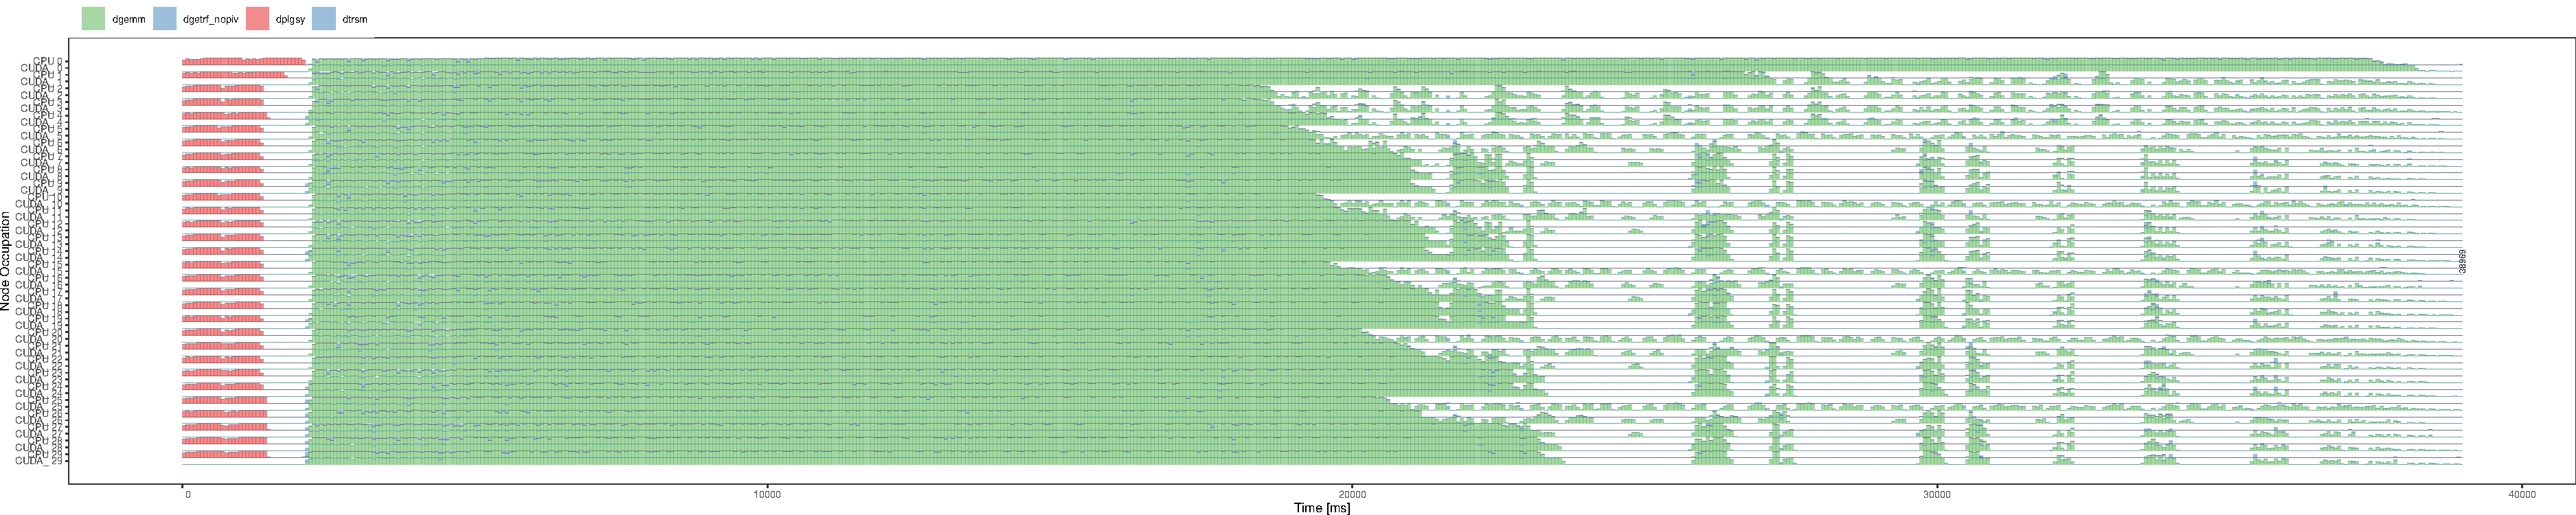
\includegraphics[height=2.5cm]{./2w+dif_original.pdf}
\end{center}

\texttt{EXAGEO}: 8 nodes, where six are CPU-only (2iters; real execution of ExaGeoStat in G5K)
\begin{center}
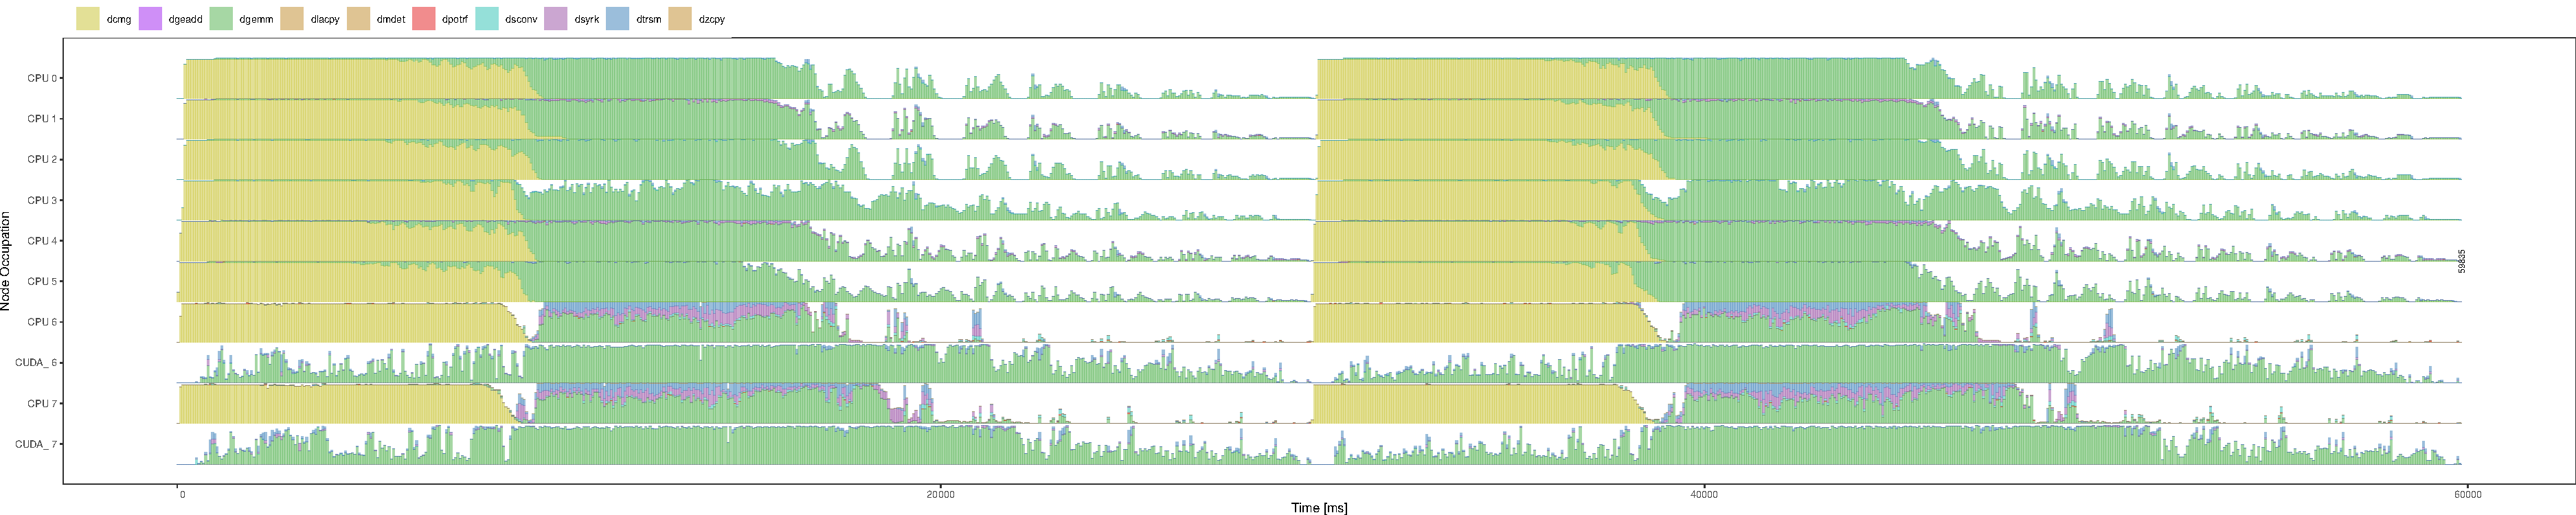
\includegraphics[height=2.5cm]{./exageo_original.pdf}
\end{center}
\end{frame}
\begin{frame}[label={sec:org2205751}]{Preliminary Results: Dense LU Facto 1/2}
StarVZ (no aggregation)  \hfill  Lpaggreg Viz (minimal aggregation)

 \hfill 100 time slices

\begin{center}
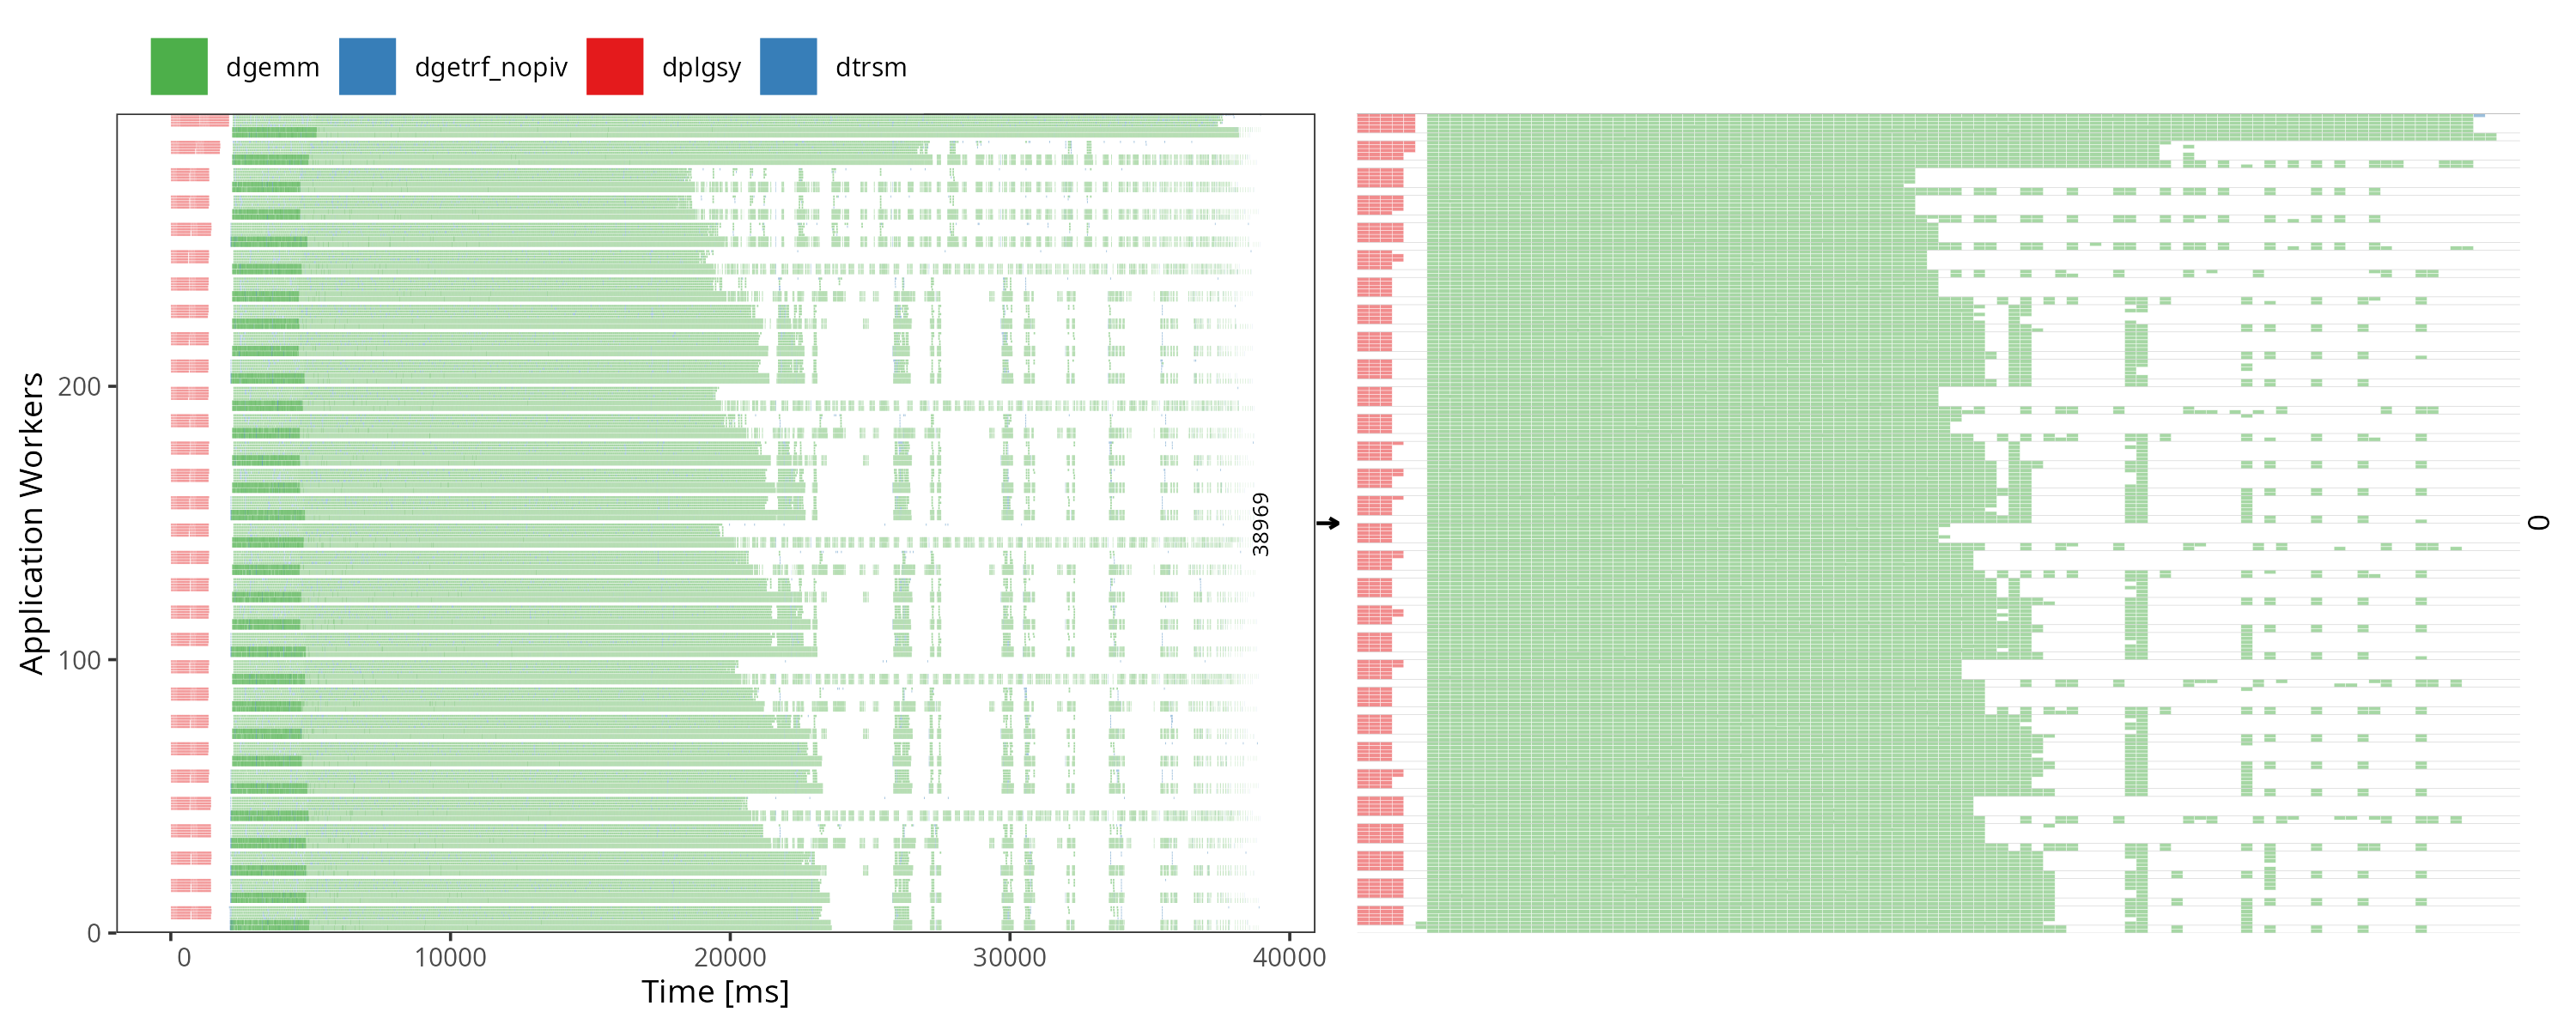
\includegraphics[width=.87\linewidth]{./2w+dif_p-0.png}
\end{center}

\vfill\pause

Overall visualization simplification (much less graphical elements)
\begin{itemize}
\item "minimal aggregation" may be more detailed with more time slices
\end{itemize}
\end{frame}
\begin{frame}[label={sec:org12c4b37}]{Preliminary Results: Dense LU Facto 2/2}
The first 10 tradeoffs (0.5 is POpt)

\begin{center}
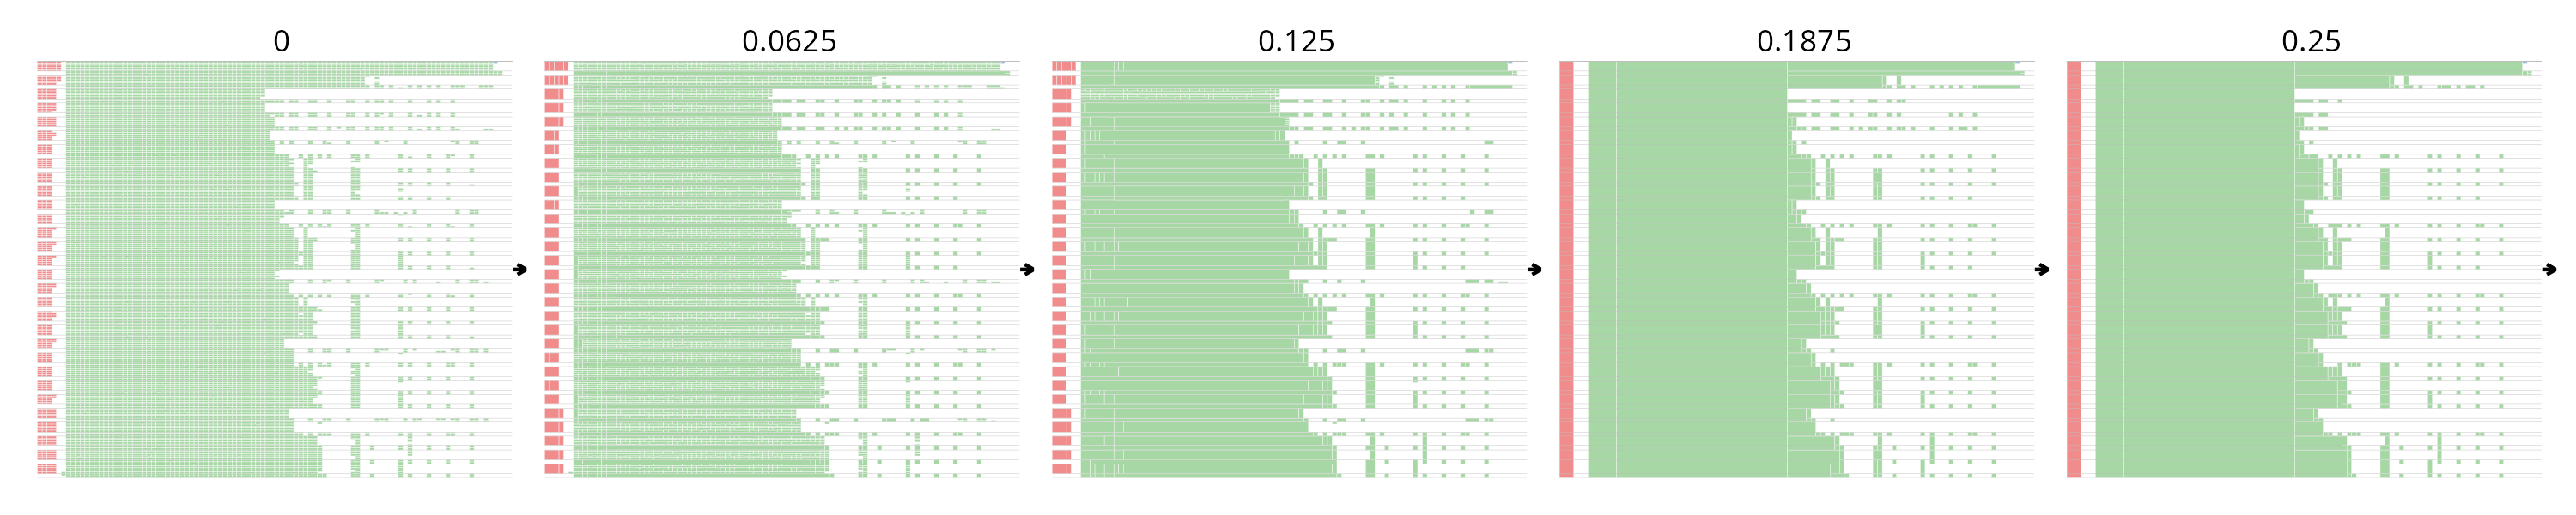
\includegraphics[width=\linewidth]{./2w+dif_5p_line1.png}
\end{center}

\begin{center}
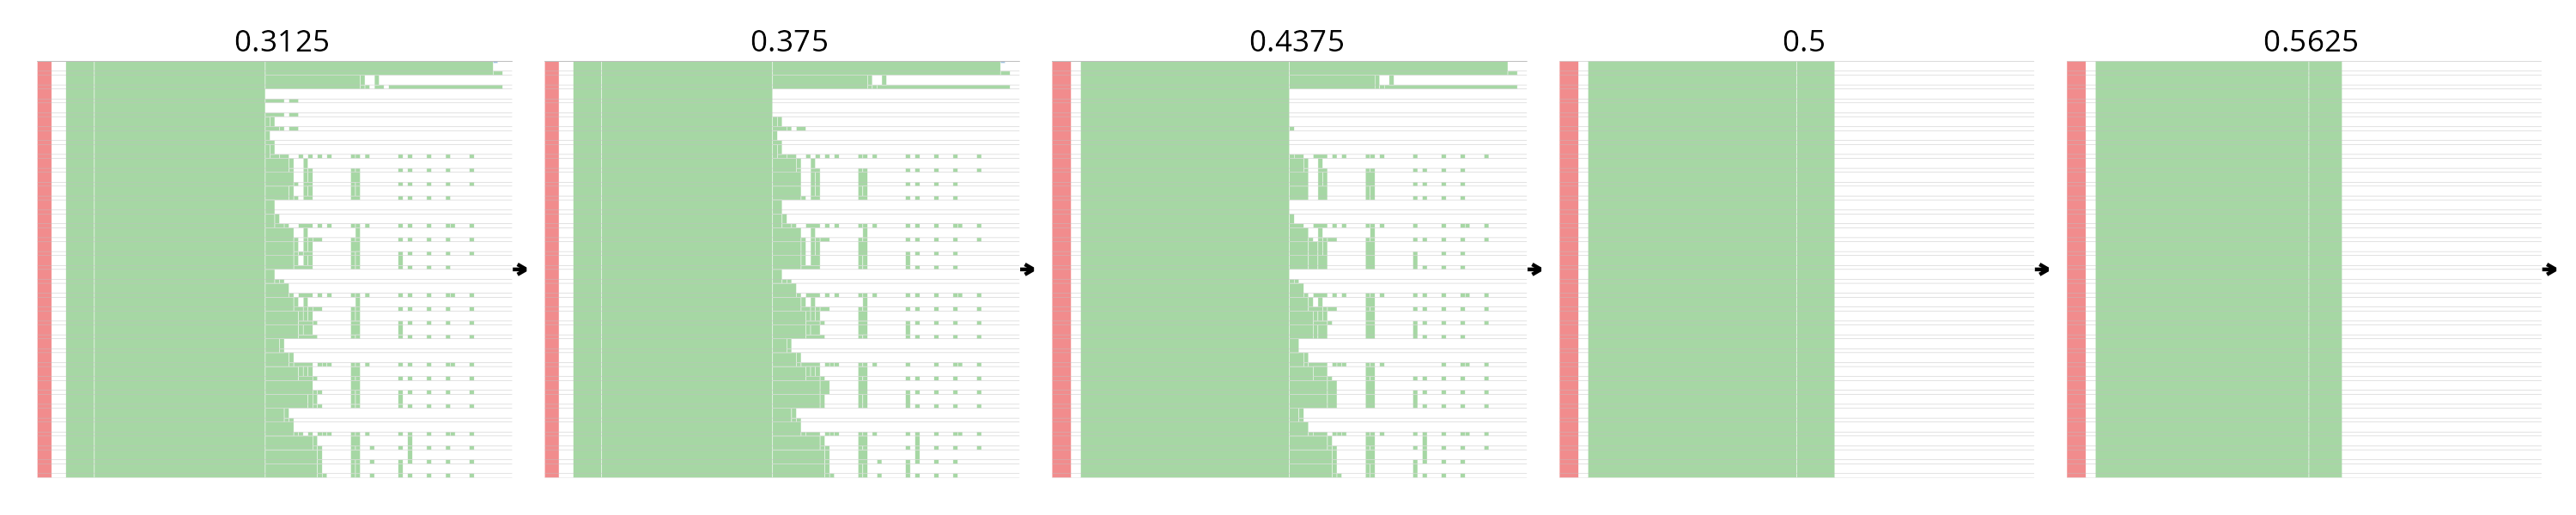
\includegraphics[width=\linewidth]{./2w+dif_5p_line2.png}
\end{center}
\end{frame}
\begin{frame}[label={sec:orgef746a3}]{Preliminary Results: ExaGeoStat 1/2}
StarVZ (no aggregation)  \hfill  Lpaggreg Viz (minimal aggregation)

 \hfill 100 time slices

\begin{center}
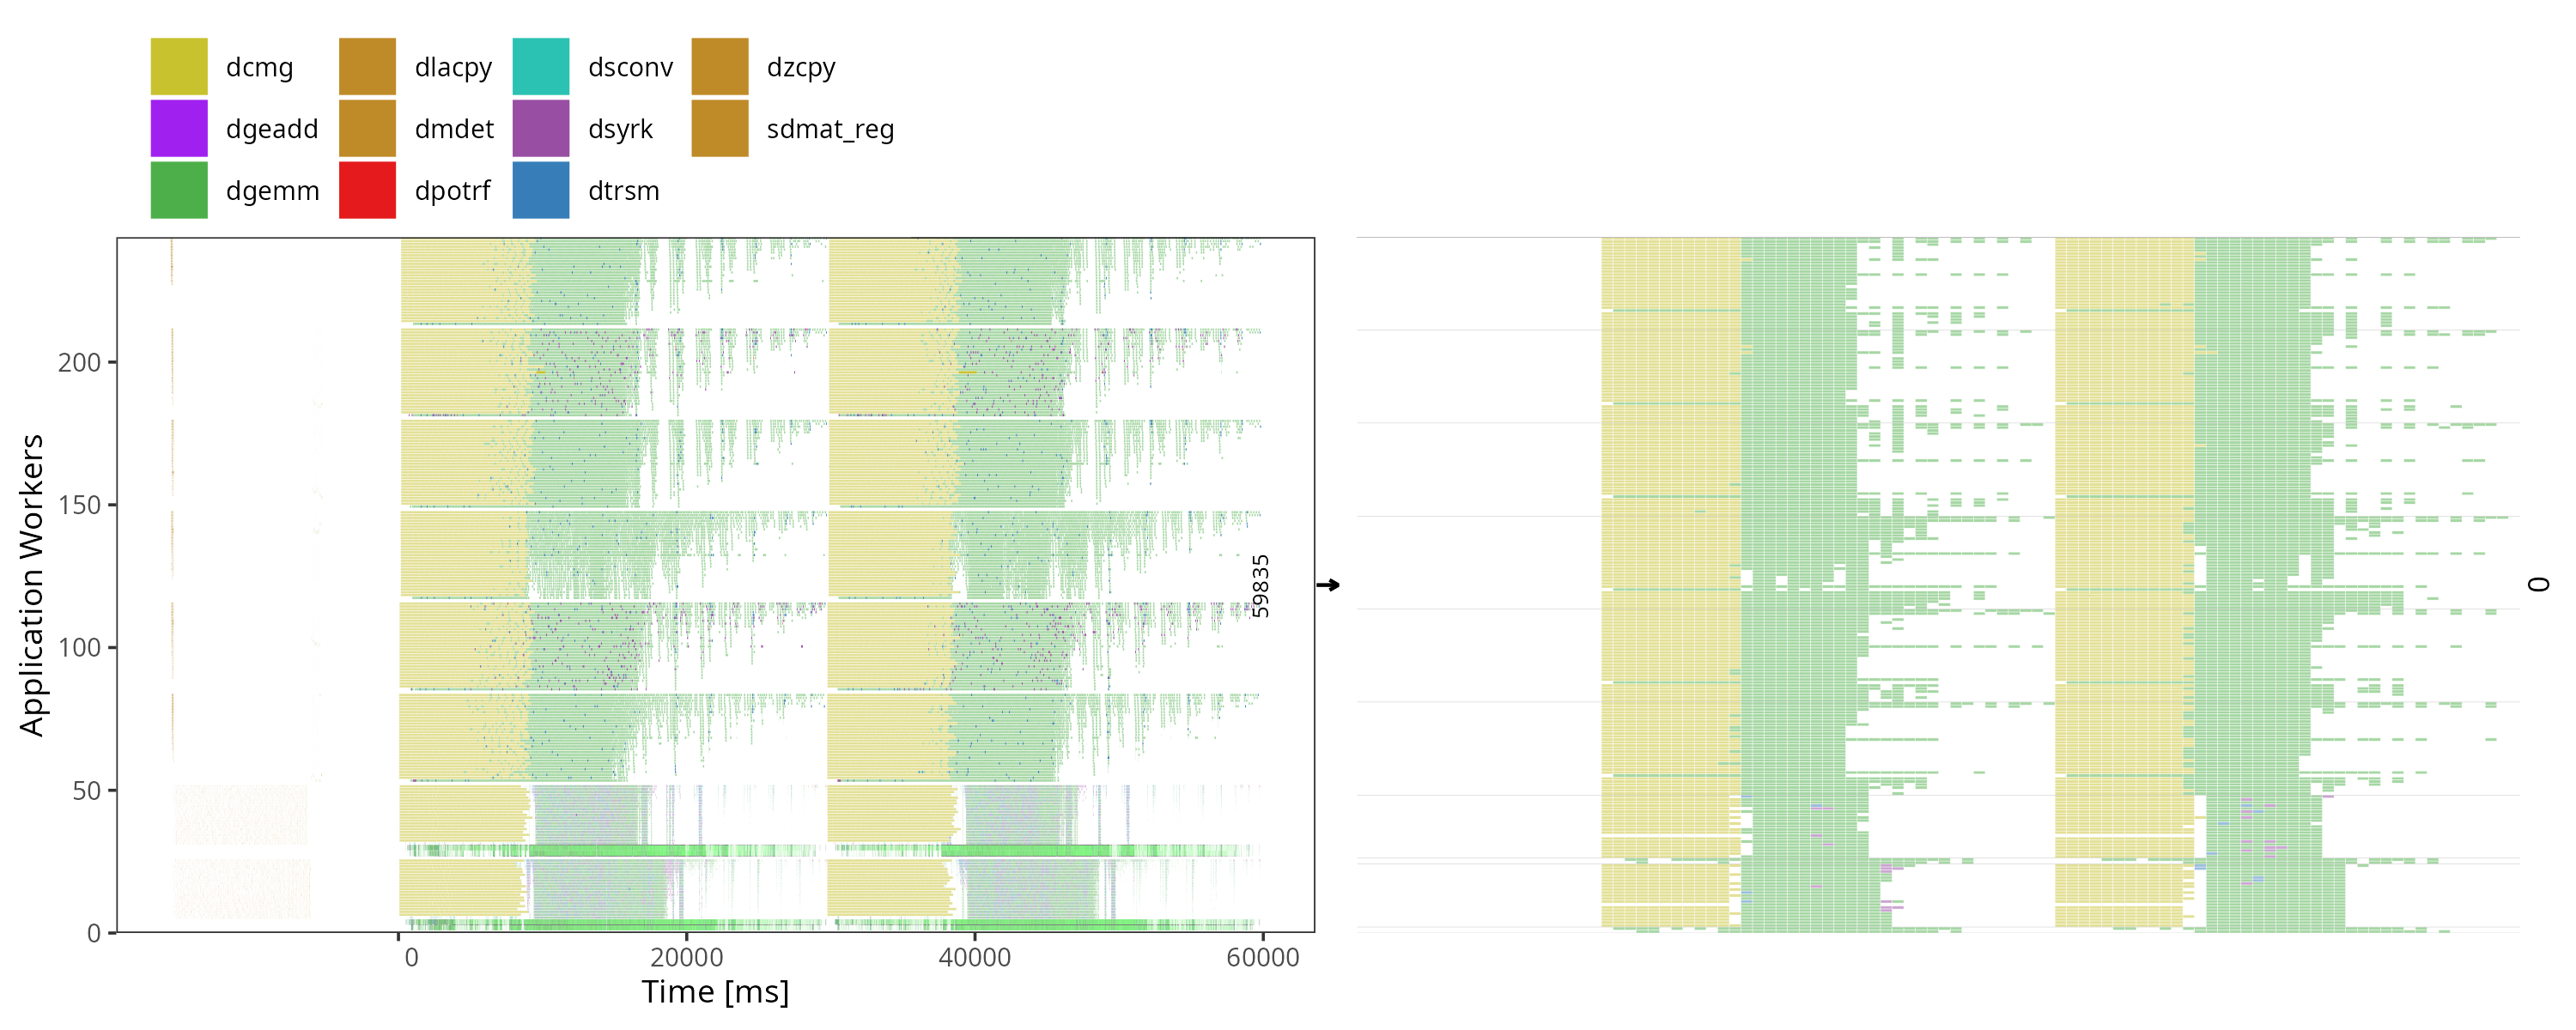
\includegraphics[width=\linewidth]{./exageo_p-0.png}
\end{center}
\end{frame}
\begin{frame}[label={sec:org15cf370}]{Preliminary Results: ExaGeoStat 2/2}
The first 10 tradeoffs (0.375 is POpt)

\begin{center}
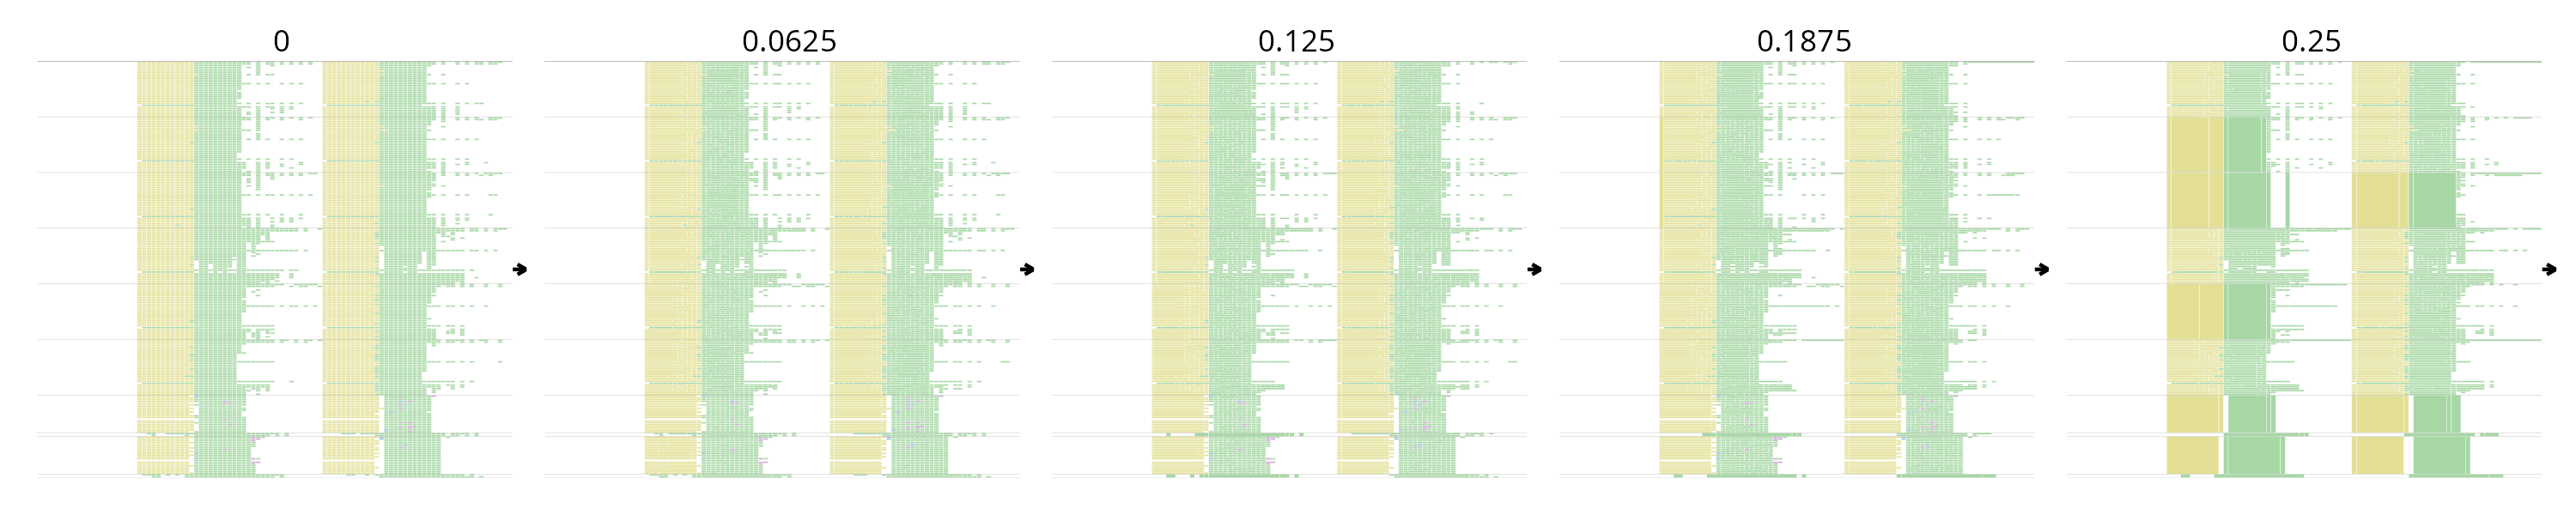
\includegraphics[width=\linewidth]{./exageo_5p_line1.png}
\end{center}

\begin{center}
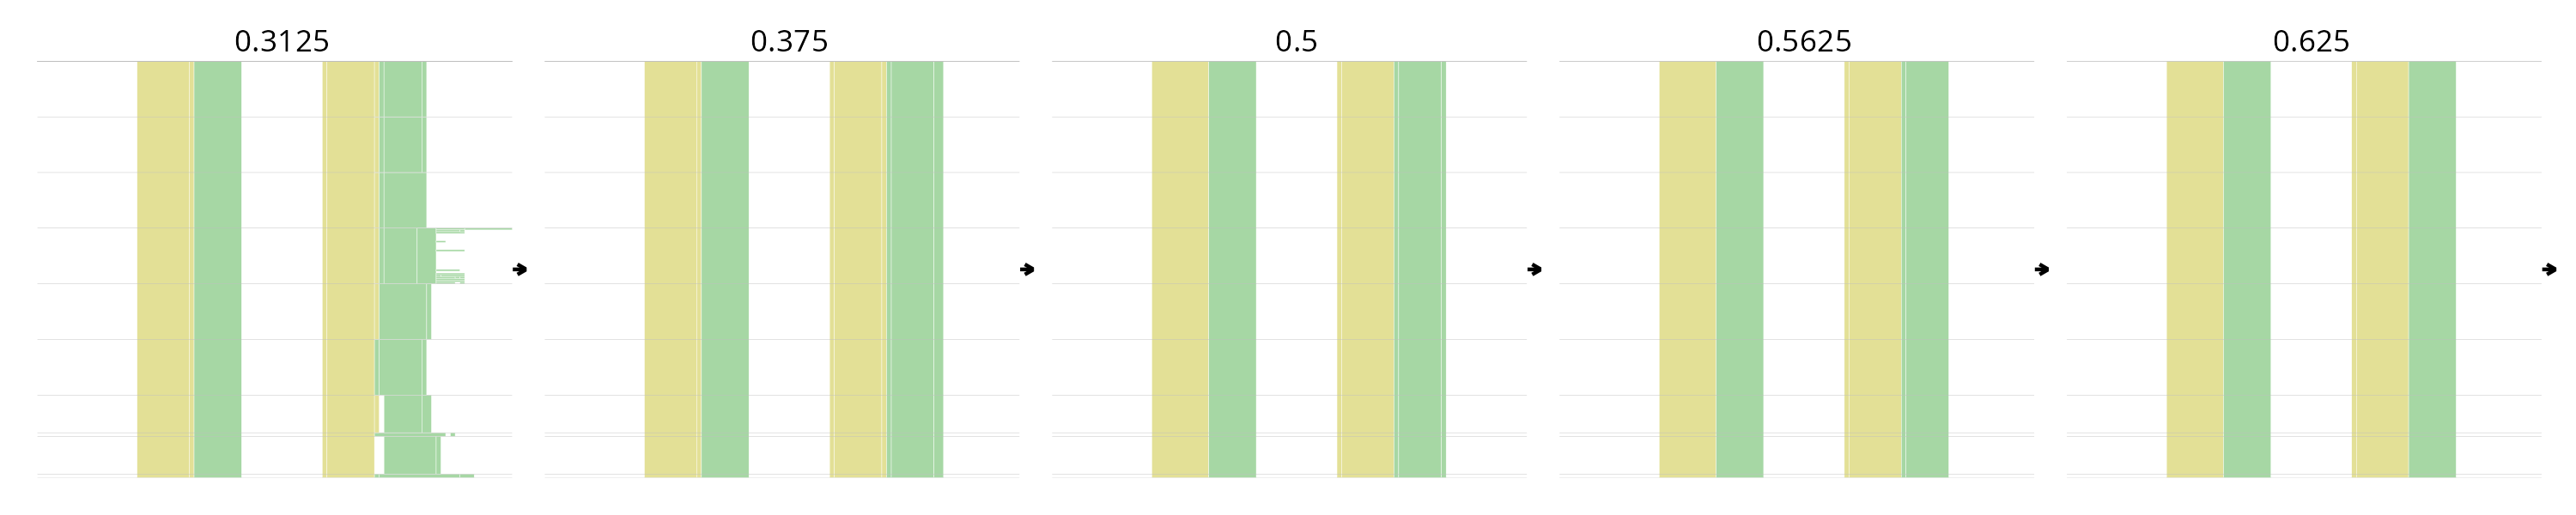
\includegraphics[width=\linewidth]{./exageo_5p_line2.png}
\end{center}
\end{frame}
\begin{frame}[label={sec:orgb44903f}]{Conclusion \& Future Work}
Weaknesses
\begin{itemize}
\item Computationally expensive (not linear) as the number of time slices increases
\begin{itemize}
\item But we can run this part in the cluster anyway
\end{itemize}
\item Method adopts a single and flat hierarchy
\begin{itemize}
\item Spatial aggregation only works with neighbor nodes
\end{itemize}
\end{itemize}

\vfill\pause

Multiple hierarchies
\begin{itemize}
\item Nesi et. al. calculates a ``Progression Metric'' for each node (PDP23)
\begin{itemize}
\item Multiple node groups with similar progressions
\end{itemize}
\item Incorporate these groups into a lpaggreg hierarchy
\begin{itemize}
\item With intermediate levels enriching the "flat" version of today
\item Slicing the trace and using several different well-selected hierarchies
\begin{itemize}
\item Surely a visualization challenge! ;-)
\end{itemize}
\end{itemize}
\end{itemize}

\vfill\pause

Machinery is working. \uline{Do some realistic performance analysis with it}.
\begin{itemize}
\item Experimentation, What-if scenarios, etc \(\to\) Large-scale experiments
\end{itemize}
\end{frame}
\begin{frame}[label={sec:org29295e7}]{Contact}
\begin{columns}
\begin{column}{0.8\columnwidth}
\begin{center}
Merci pour votre attention !
\end{center}

\begin{center}
Lucas Mello Schnorr <schnorr@inf.ufrgs.br>

Lucas Barros de Assis <lucas.assis@inf.ufrgs.br>
\end{center}
\end{column}
\begin{column}{0.2\columnwidth}
\begin{center}

\includegraphics[width=\linewidth]{./img/qrcode.png}
\end{center}
\end{column}
\end{columns}
\end{frame}
\end{document}
